
\section{CPVR - CAVE}
Die Forschungsgruppe \textit{Computer Perception \& Virtual Reality} der Berner Fachhochschule f"ur Technik und Informatik, betreibt einen 4-Wand CAVE (CAVE Automatic Virtual Environment) f"ur die Visualisierung und Simulation von Projekten im medizinischen Umfeld.

Ein CAVE bezeichnet einen Raum zur Projektion einer dreidimensionalen Illusionswelt der virtuellen Realit"at. Dieser Raum kann auf verschiedene Weisen realisiert werden. Im Falle der CPVR Forschungsgruppe handelt es sich um einen offenen W"urfel, bestehend aus 4 W"anden: einer Frontwand, zwei Seitenw"anden und einem Boden. Bei den drei W"anden handelt es sich um R"uckprojektionsleinw"ande, die in einem Kubus angeordnet sind. Auf jede R"uckwand wird mittels zweier Projektoren ein stereoskopisches Bild projeziert, welches durch einen Computer erzeugt wird. Zwischen den Projektionsfl"achen nimmt der Benutzer mit einer Stereobrille eine dreidimensionale virtuelle Umgebung wahr, in der er sich mit Hilfe verschiedener Eingabeger"ate frei bewegen kann. Weiter wird ein Tracker eingesetzt. Falls sich ein Benutzer im virtuellen Raum bewegt, so bewegen sich die Objekte mit. Mit dem eingebauten Tracker wird erfasst wohin ein Benutzer schaut. Mit diesen Angaben berechnet der CAVE-Server anschliessed die Korrektur, damit die virtuellen Objekte scheinbar station"ar bleiben.

Die vierte Projektionsfl"ache - der Boden - ist erst seit kurzem in Betrieb. Anders als bei den W"anden, wird beim Boden nicht von ausserhalb des W"urfels projeziert, sondern von der Decke. Mit dem Boden als weitere Projektionsfl"ache kann eine wesentlich bessere Immersion erreicht werden.
Die Projektoren f"ur die Bodenfl"ache sind an der Decke befestigt. Damit m"oglichst wenig Schatten auf die Projektionsfl"ache fallen, wird das Bild etwas geneigt von vorne projiziert. So fallen die Schatten hinter den Betrachter und beeinflussen die Immersion weniger. Dies bedingt jedoch, dass sich immer nur eine Person im CAVE befindet und diese nicht nach hinten schaut.

\begin{figure}[ht]
\begin{center}
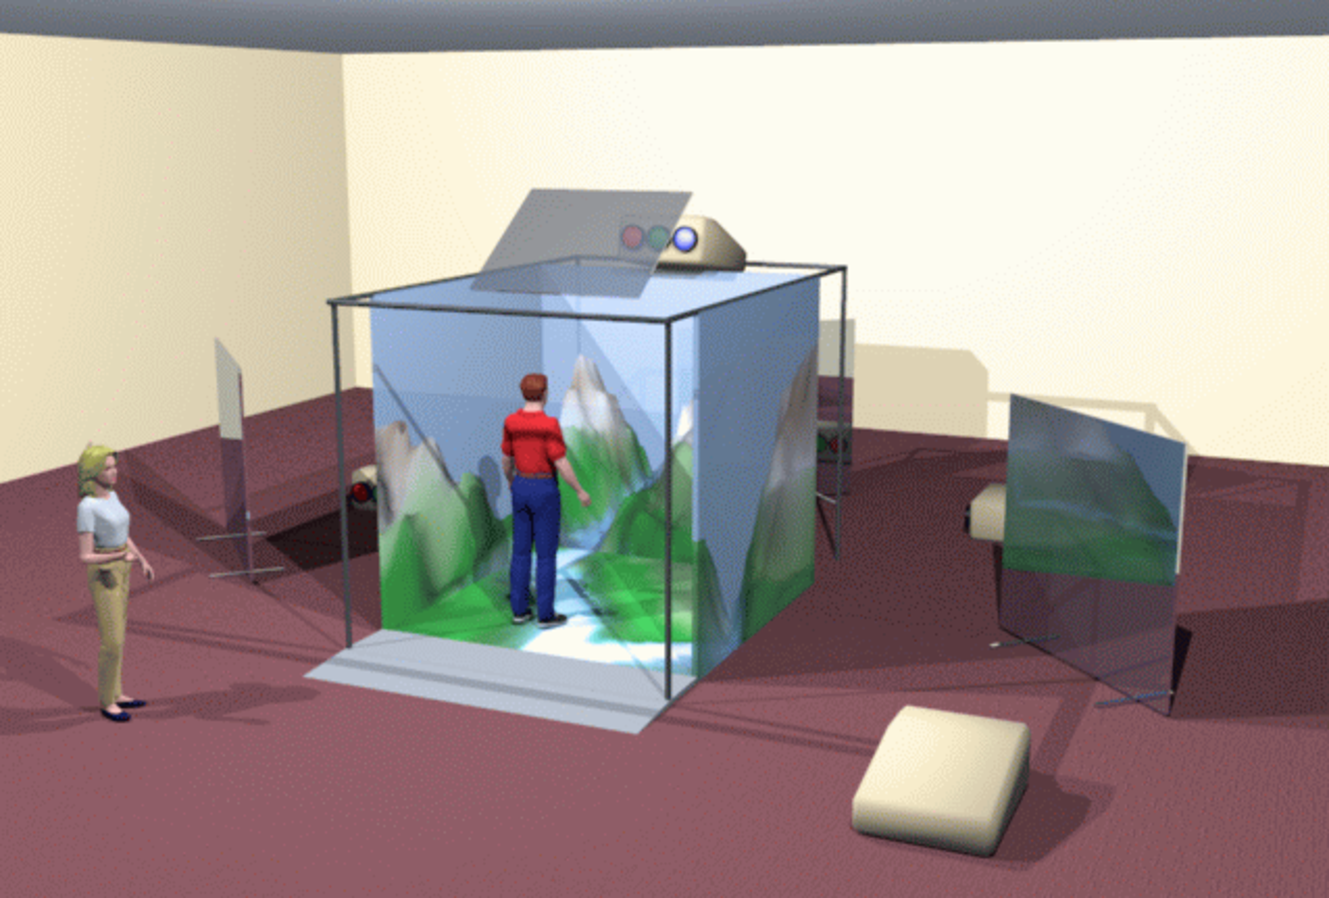
\includegraphics[scale=0.4]{../figures/cave_lab}
\end{center}
\caption{CAVE Lab (Quelle: [4])}
\end{figure}

\subsection{Konfiguration}
Der CAVE wird mit einem Server und acht Render Clients betrieben, die "uber ein Ethernet Netzwerk kommunizieren. Der Server ist verantwortlich f"ur die Koordination der Render Clients. Die Render Clients berechnen die Bilder und stellen diese dar. "Uber den digitalen Videokanal (DVI) werden die Projektoren an die Rendering Clients angeschlossen. Die Projektoren lassen sich "uber eine RS232C Schnittstelle von einem PC aus steuern. An einem Render Client sind per daisy chain von je zwei Projektoren angeschlossen. Abbildung \ref{cave_config} ist eine vereinfachte Darstellung, welche den CAVE mit nur drei W"anden zeigt.

\begin{figure}[ht]
\begin{center}
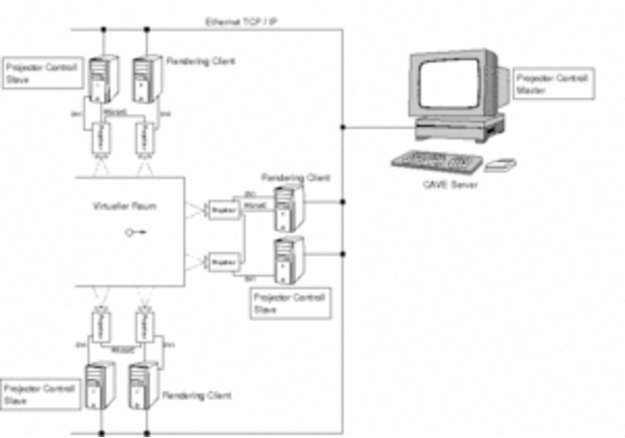
\includegraphics[scale=0.5]{../figures/cave_config}
\end{center}
\caption{CAVE Config f"ur drei W"ande (Quelle: [4])}
\label{cave_config}
\end{figure}

\subsection{Stereoskopie}
Um ein stereoskopisches Bild zu erzeugen, m"ussen zwei Bilder von zwei Projektoren gleichzeitig "ubereinander auf die gleiche Leinwand projeziert werden. Die Bilder der beiden Projektoren werden exakt parallel auf die Leinwand projeziert. Der mechanische Abstand der beiden Projektionsquellen muss softwareseitig korrigiert werden, d.h. die Bilder werden "ubereinander geschoben. Die Projektoren verf"ugen "uber eine spezielle Firmware Version (901.2202.41), welche die Positionierung des Bildes unterst"utzt. Dabei wird die maximale Hardwareaufl"osung von 1400x1050 softwarem"assig auf 1280x1024 reduziert.

Der somit entstandene Rand kann f"ur die Positionierung des Bildes gebraucht werden. Die Bilder lassen sich mit dieser Funktion pixelgenau "ubereinander positionieren.


\begin{figure}[ht]
\begin{center}
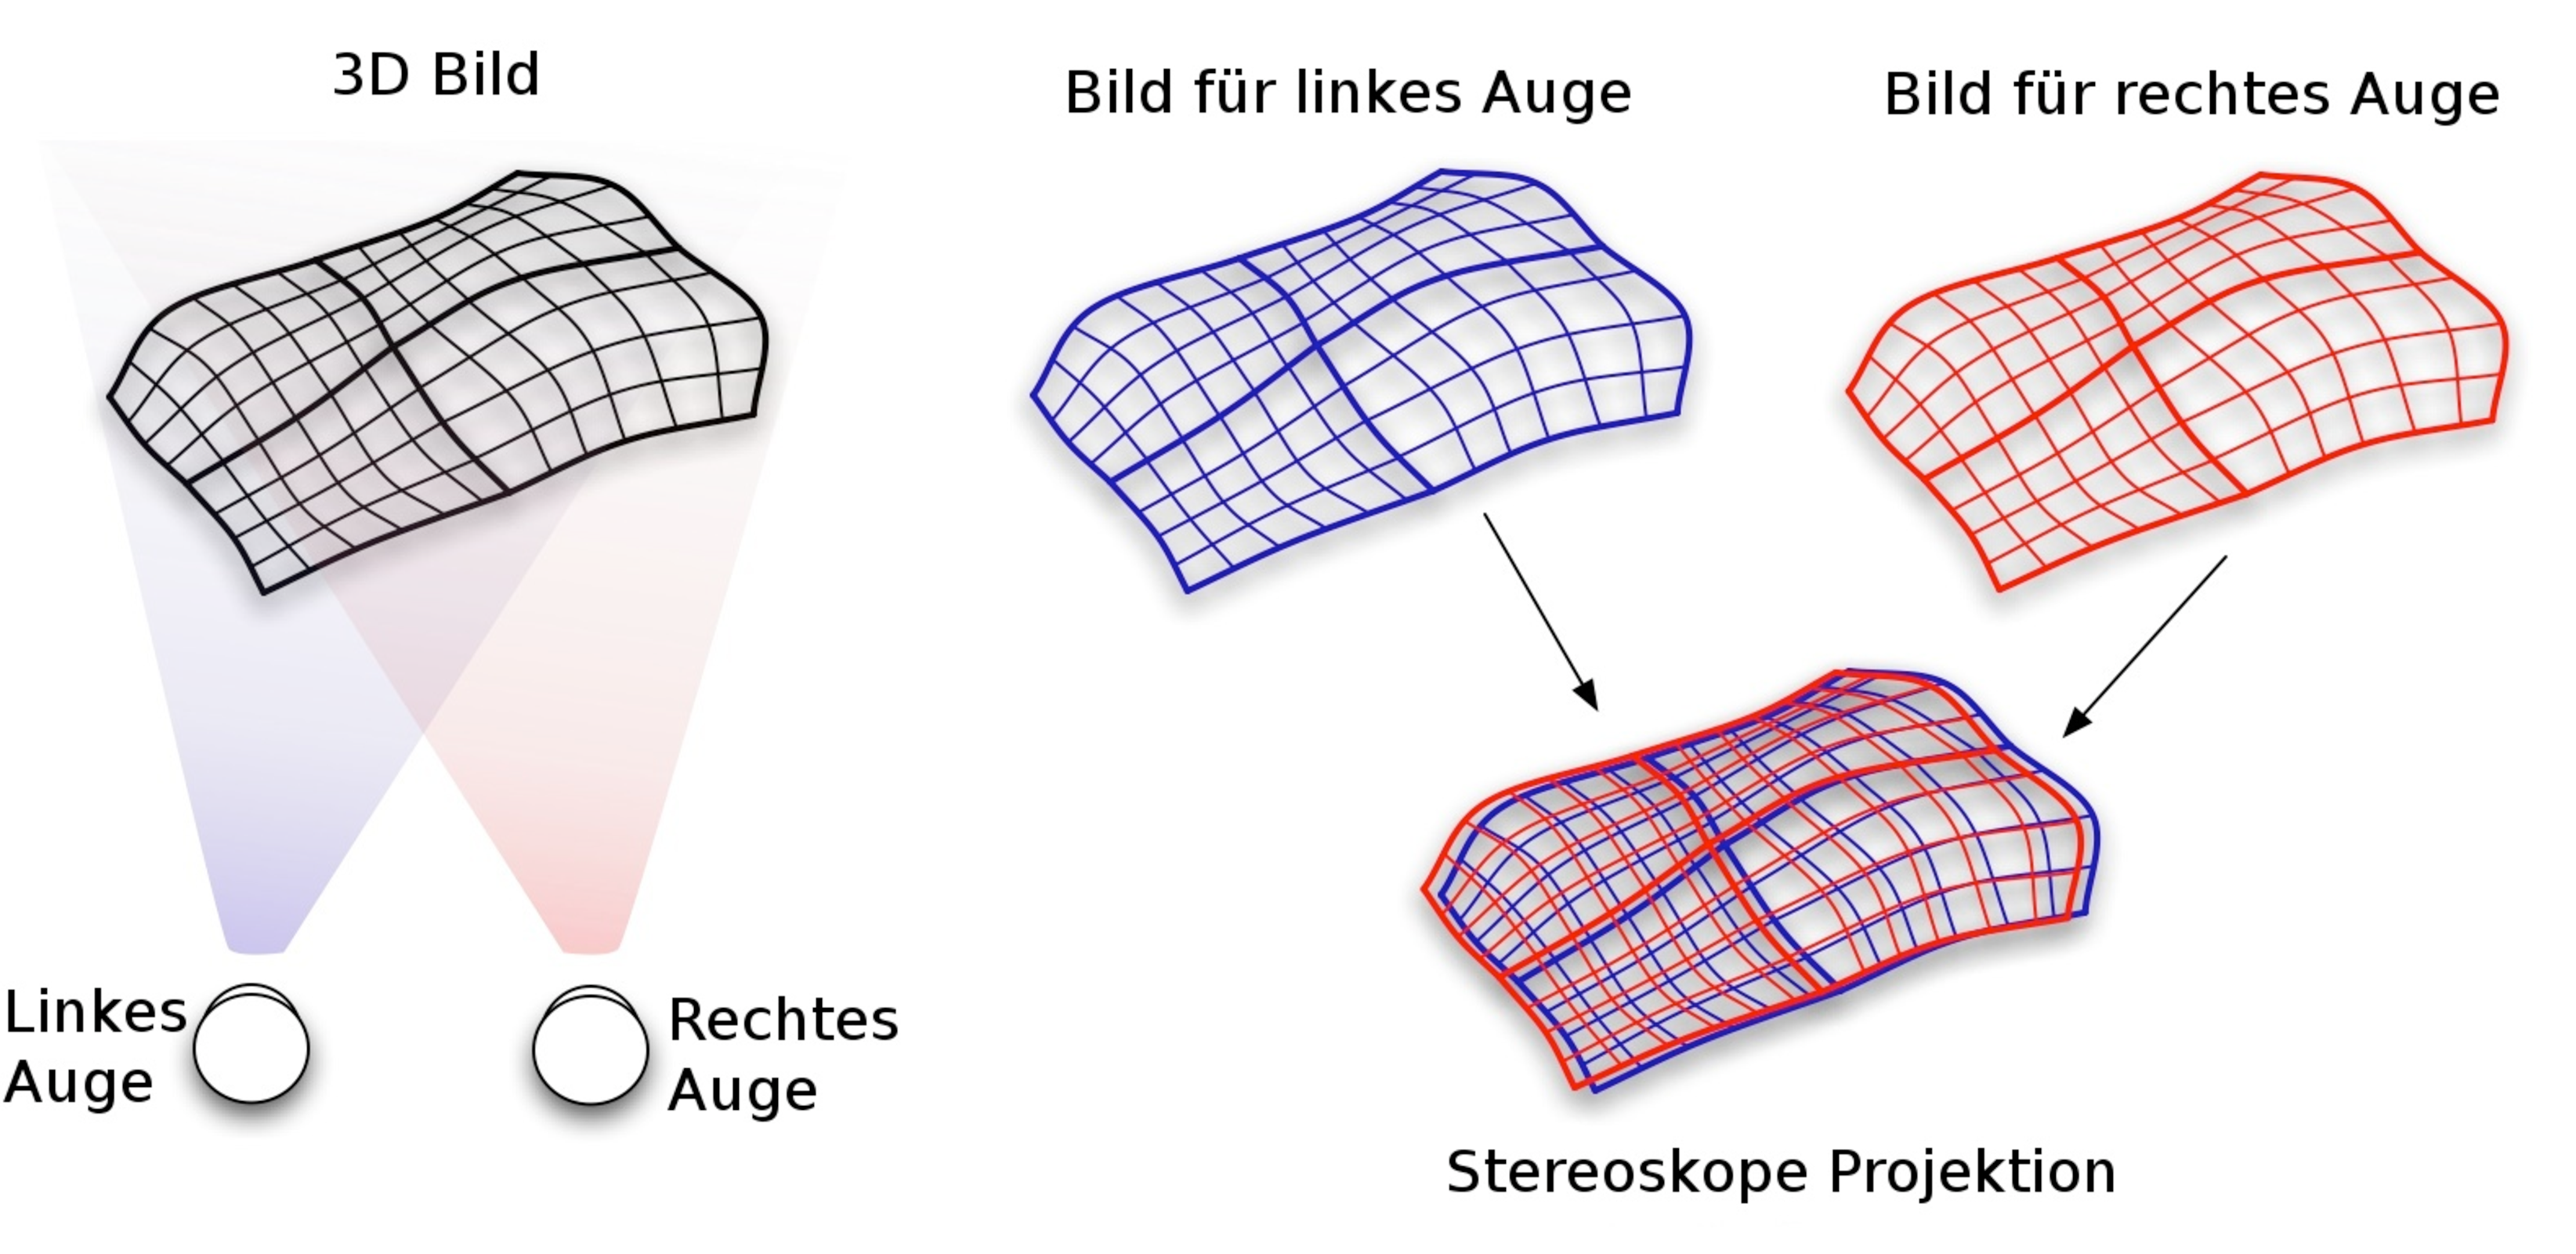
\includegraphics[scale=0.2]{../figures/stereoscopy}
\end{center}
\caption{Stereoskopie}
\end{figure}
